% Copyright 2004 by Till Tantau <tantau@users.sourceforge.net>.
%
% In principle, this file can be redistributed and/or modified under
% the terms of the GNU Public License, version 2.
%
% However, this file is supposed to be a template to be modified
% for your own needs. For this reason, if you use this file as a
% template and not specifically distribute it as part of a another
% package/program, I grant the extra permission to freely copy and
% modify this file as you see fit and even to delete this copyright
% notice. 

\documentclass{beamer}

% There are many different themes available for Beamer. A comprehensive
% list with examples is given here:
% http://deic.uab.es/~iblanes/beamer_gallery/index_by_theme.html
% You can uncomment the themes below if you would like to use a different
% one:
%\usetheme{lankton-keynote}
%\usetheme{AnnArbor}
%\usetheme{Antibes}
%\usetheme{Bergen}
%\usetheme{Berkeley}
%\usetheme{Berlin}
%\usetheme{Boadilla}
%\usetheme{boxes}
%\usetheme{CambridgeUS}
%\usetheme{Copenhagen}
%\usetheme{Darmstadt}
%\usetheme{default}
%\usetheme{Frankfurt}
%\usetheme{Goettingen}
%\usetheme{Hannover}
%\usetheme{Ilmenau}
%\usetheme{JuanLesPins}
%\usetheme{Luebeck}
\usetheme{Madrid}
\usepackage[final]{pdfpages}
%\usetheme{Malmoe}
%\usetheme{Marburg}
%\usetheme{Montpellier}
%\usetheme{PaloAlto}
%\usetheme{Pittsburgh}
%\usetheme{Rochester}
%\usetheme{Singapore}
%\usetheme{Szeged}
%\usetheme{Warsaw}
%\usecolortheme{beetle}

\newcommand*\samethanks[1][\value{footnote}]{\footnotemark[#1]}

\setbeamertemplate{navigation symbols}{}%remove navigation symbols
\title[The Network of FDI Flows]{The Network of Foreign Direct Investment Flows:\\Theory and Empirical Analysis\thanks{\footnotesize {Acknowledgement: This material is based on work supported by the National Science Foundation under IGERT Grant DGE-1144860, Big Data Social Science.}}}


\author[J.\,Schoeneman, B. \,Zhu \& B.\,Desmarais]{%
  \texorpdfstring{%
    \begin{columns}
      \column{.3\linewidth}
      \centering
      John Schoeneman{\thanks{Pennsylvania State University}} \\ \small{jbs5686@psu.edu\\ PhD Candidate}
      \column{.3\linewidth}
      \centering
      Boliang Zhu{\samethanks[2]} \\ \small{bxz14@psu.edu\\ Assistant Professor}
    \end{columns}
    \vspace{12pt}
    \begin{columns}
      \column{.3\linewidth}
      \centering
      Bruce Desmarais{\samethanks[2]}\\ \small{bdesmarais@psu.edu\\ Associate Professor}
    \end{columns}
 }
 {Author 1, Author 2, Author 3}
}

\date{April 8, 2017}



% - Use the \inst command only if there are several affiliations.
% - Keep it simple, no one is interested in your street address.

% - Either use conference name or its abbreviation.
% - Not really informative to the audience, more for people (including
%   yourself) who are reading the slides online


% This is only inserted into the PDF information catalog. Can be left
% out. 

% If you have a file called "university-logo-filename.xxx", where xxx
% is a graphic format that can be processed by latex or pdflatex,
% resp., then you can add a logo as follows:

% \pgfdeclareimage[height=0.5cm]{university-logo}{university-logo-filename}
% \logo{\pgfuseimage{university-logo}}


% Let's get started
\begin{document}

\begin{frame}
  \titlepage
\end{frame}


% Section and subsections will appear in the presentation overview
% and table of contents.


\begin{frame}{Introduction}

\frametitle{Introduction}
  \begin{columns}[T]
    \begin{column}{.5\textwidth}
\vspace{10mm}
\begin{itemize}
\item{FDI as a Network}
\begin{itemize}
\item{Clustering}
\item{Reciprocity}
 \end{itemize}
 \item{Motivation}
 \begin{itemize}
\item{Violation of Independence Assumptions}
\item{Theoretical Importance of Dependence Terms}
 \end{itemize}
  \item{Simultaneously test exogenous variables as well}
 \end{itemize}
    \end{column}
    \begin{column}{.5\textwidth}
    \begin{block}{FDI Network 2008}
    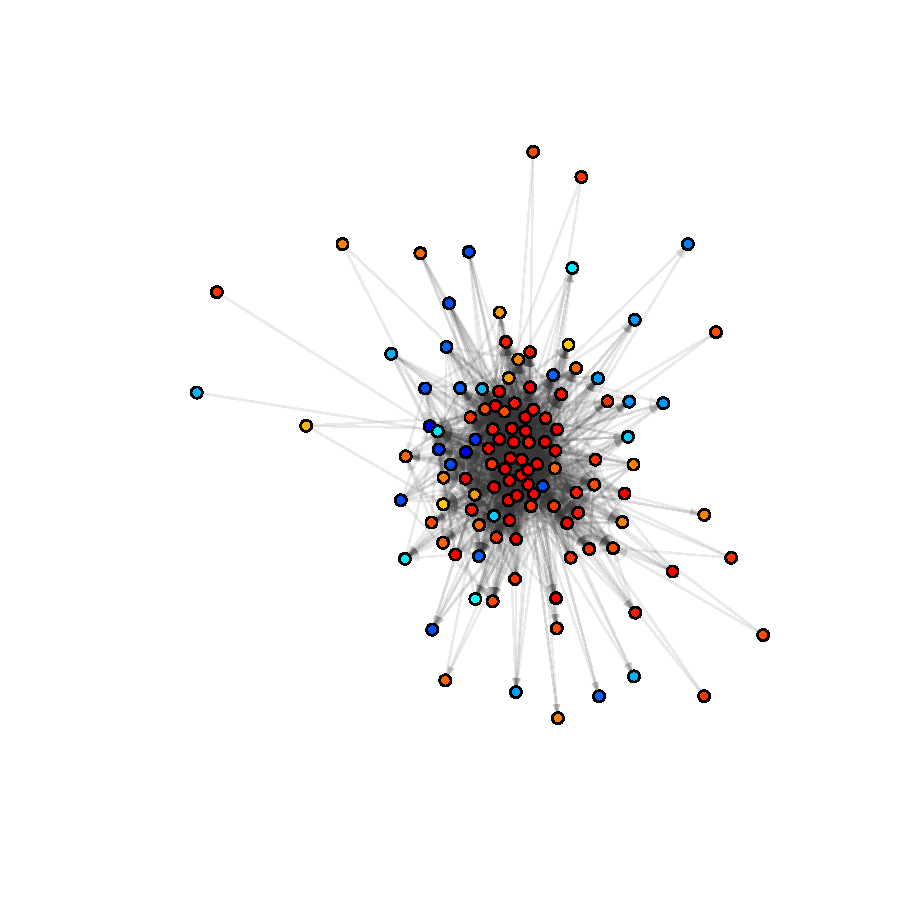
\includegraphics[scale=.4]{slides_figures/fdiNet2008.pdf}
 \small{\\ Color Scheme: Autocracy to Democracy is scaled as Blue to Red}
    \end{block}
    \end{column}
  \end{columns}

%In the image on the right is the network for weighted FDI flows for 2008. There are a couple things that are immediately obvious. The first is that we clearly see clustering. This clustering is based on FDI flows, which are the ties for between nodes, which here are countries. The more ties a node has and the larger these ties are, the more centrally placed a node is and the more shared partners and size of edge they share with a node, the closer they are to that node. This clear dependence in structure motivates us to model these networks, both to eliminate the potential bias that comes from ignoring them and measure the dependence , which we argue has theoretical importance. The second point is that it appears Polity plays a role in clustering as well, with red, democratic nodes often close to one another. Network models allow us to test exogenous variables such as the role of regime type alongside of network terms, and so we focus on both political and economic variables that have been estimated in the past, but in standard regression models that assumed independence.

\end{frame}

\begin{frame}{Theory for Network Terms}

% Why reciprocity

% Why transitivity 

\end{frame}

\begin{frame}{Exogenous Covariates}

%Dyad:  Gravity, Contiguity, Common Language, Four types of treaty, PTA depth, Colonial Relationship, 
%Node: GDPpc, growth rate, Polity, PV, and trade openness
 
\end{frame}



\begin{frame}{Data}

% where bilateral data comes from
% gravity model 
% list of covariates

\end{frame}

\begin{frame}{Network Statistics}

% Network measurements and what they mean

\end{frame}


\begin{frame}{ERGM Count Model}

% General explanation of ERGM
	% How does this solve the problem of dependences
% How network terms are estimated
% How Exogenous Variables are included

\end{frame}

\begin{frame}{Results}

% Model Specfication

\end{frame}


\begin{frame}{Conclusion and Future Research}

\end{frame}


\begin{frame}{References}


\end{frame}




\end{document}




